\documentclass{beamer}

%style
\mode<presentation>
\usetheme{Boadilla}

%Packages
\usepackage[utf8]{inputenc}
\usepackage[ngerman]{babel}
\usepackage{graphicx}
\usepackage{booktabs}
\usepackage{mathtools}
\usepackage{amsmath}
\usepackage{listings}
\usepackage[utf8]{inputenc}
\usepackage[ngerman]{babel}
\usepackage[T1]{fontenc}
\usepackage{lmodern}
\usepackage{tabto}
\usepackage{listings}
\usepackage{framed} 
\usepackage{xcolor} 
\colorlet{shadecolor}{gray!25}
%bibtex
\usepackage[backend=biber, style=authoryear]{biblatex}
\addbibresource{referenzen.bib}

%Einstellungen der Präsentation
\title[Cybersecurity]{Flubot:\\ Android-Malware verbreitet sich über Fake-Patches\\!WIP!}
\author{Moritz Rupp}
\institute[MR]{Hochschule Albstadt-Sigmaringen}

\date{tobedated - WS 21/22}

%Beginn der Präsentation
\begin{document}

%Titelseite
\begin{frame}
\titlepage
\end{frame}
%Inhaltsverzeichnis
\begin{frame}
\frametitle{Inhalt}
\tableofcontents    
\end{frame}
\begin{frame}{Leitartikel}
\begin{center}
 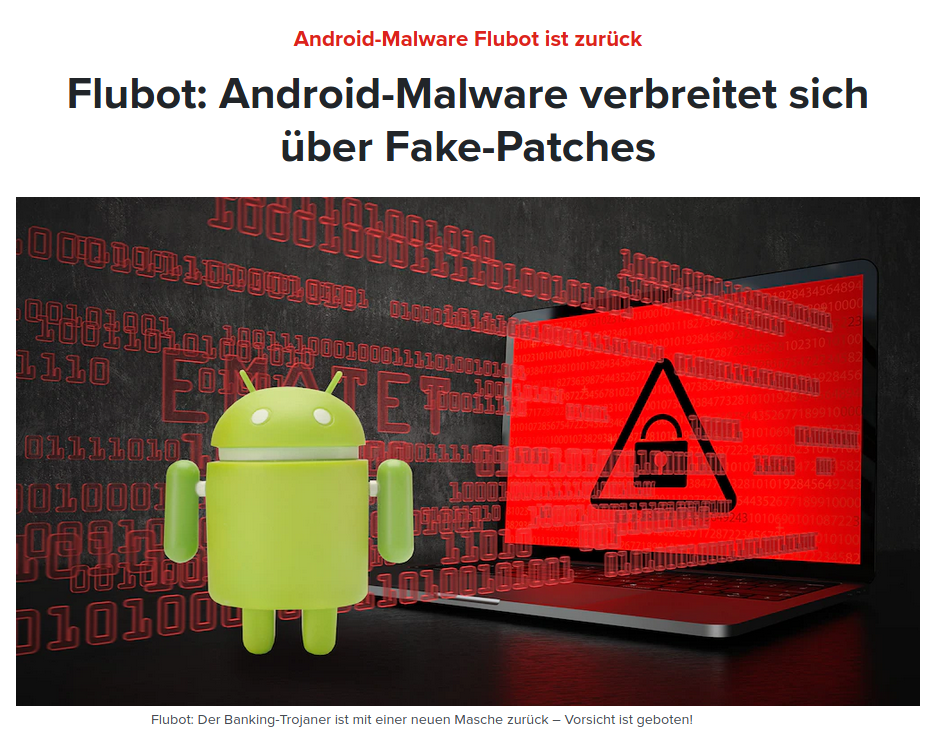
\includegraphics[scale=0.31]{bild.png} 

\end{center}

\end{frame}

\begin{frame}{Trivia}
 \section{Trivia}
 \begin{itemize}
  \item Banking Trojaner - Phishing Malware
  \item Erstes Auftreten Ende 2020 in Spanien\\
  	- Frühjar 2021 in Deutschland
  \item 80 tausend Infizierte Geräte
  \item im Umlauf
  \item Schaden in höhe von 10 Mio €
 \end{itemize}
\end{frame}
\begin{frame}{Was ist Flubot?}
- Verbreitung über SMS \\
- kurzer Text mit Link\\
- vermeintlicher Dienst wie Voicemail etc. \\
- Nur durch herunterladen der apk nutzbar\\

\begin{block}{Banking Trojaner}
 Vermeintlich harmlose Anwendung dringt in System ein und\\
 greift Daten ab.\\
 - In diesem Fall Banking Apps
\end{block}
\begin{block}{Botnetze}
 Große Anzahl an Infizierten Geräten die automatisiert Malware betreiben und sich verbreiten
\end{block}

\end{frame}
\section{Funktionsweiße}
\begin{frame}{Funktionsweiße}
-Opfer erhählt eine SMS mitsamt Link!\\
-Der Link führt zu einer Webseite auf der ein APK Download zu verfügung gestellt wird.\\
- Durch Download der APK wird das betroffene Gerät infiziert!\\
- Die Malware durchsucht nun die Kontaktliste und schickt über diese weitere Phishing Nachrichten!\\
- Des weiteren werden über Banking Apps Phishing Overlays gelegt!\\
$\Rightarrow$ Jegliche Eingaben werden nun seitens der Angreifer mitgelesen!
\end{frame}
\section{Verbreitung}
\begin{frame}{Verbreitung}
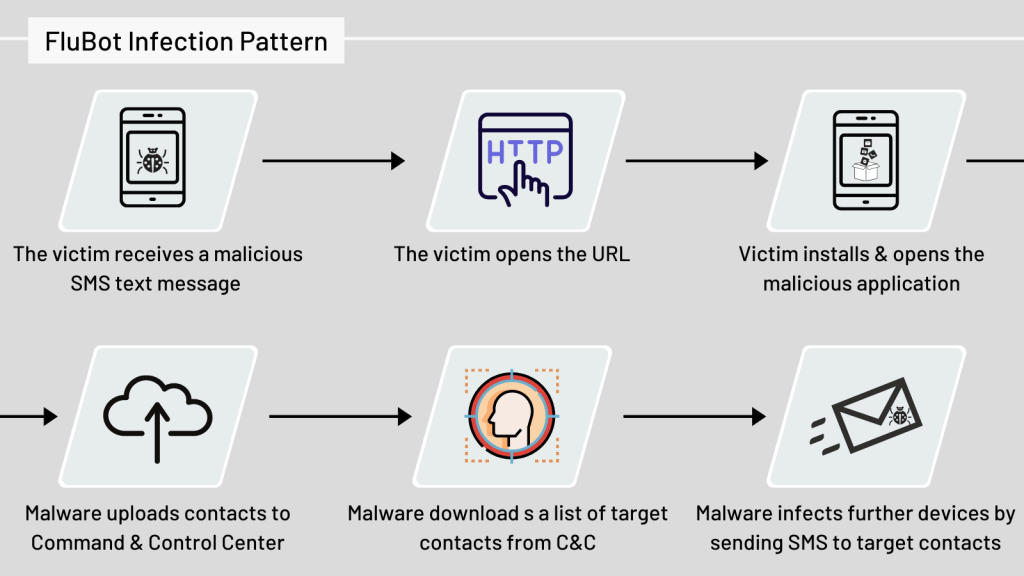
\includegraphics[scale=0.41]{command_control_server.png}
\end{frame}
\subsection{Phishing}
\begin{frame}{Phishing}
- Anfangs wird eine vermeintliche Voicemail als Köder verwendet!\\
- Seit Anfang 2021 Packetlieferdienste!\\
- Seit mitte 2021 Fake security update gegen Flubot selbst!
\end{frame}
\begin{frame}
\begin{center}
 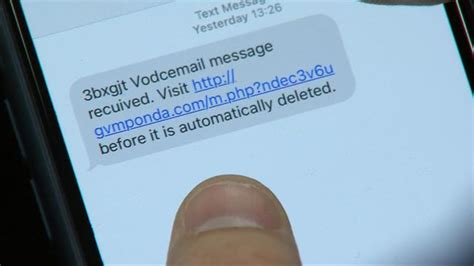
\includegraphics[scale=0.51]{voice.jpeg}

\end{center}
\end{frame}
\begin{frame}
\begin{center}
 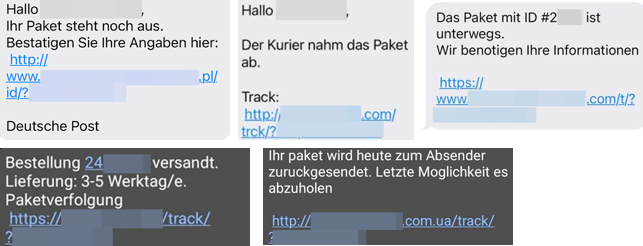
\includegraphics[scale=0.51]{external-content.duckduckgo.com.png}

\end{center}


\end{frame}
\begin{frame}
\begin{center}
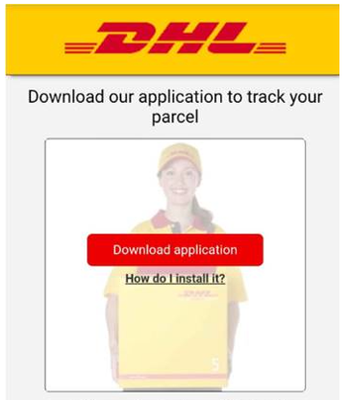
\includegraphics[scale=0.51]{dhl.png}

\end{center}


\end{frame}

\begin{frame}{Post-Infection}
 - Verbindungsaufbau zum Command and Control Server!\\
\begin{block}{Command and Control Server}
Hauptzentrale des Botntzes! Hier wird die Malware gesteuert!
\end{block}
- Infiziertes Gerät schickt alle Kontakte und installierten Apps an den C\&C Server!\\
- Dieser Antwortet mit einer neuen Liste Kontakte!\\
- Über diese wird die Malware nun weiter verbreitet!\\
- Auch wird eine Liste der gezielten Anwendungen geschickt!
\end{frame}
\begin{frame}
\begin{center}
 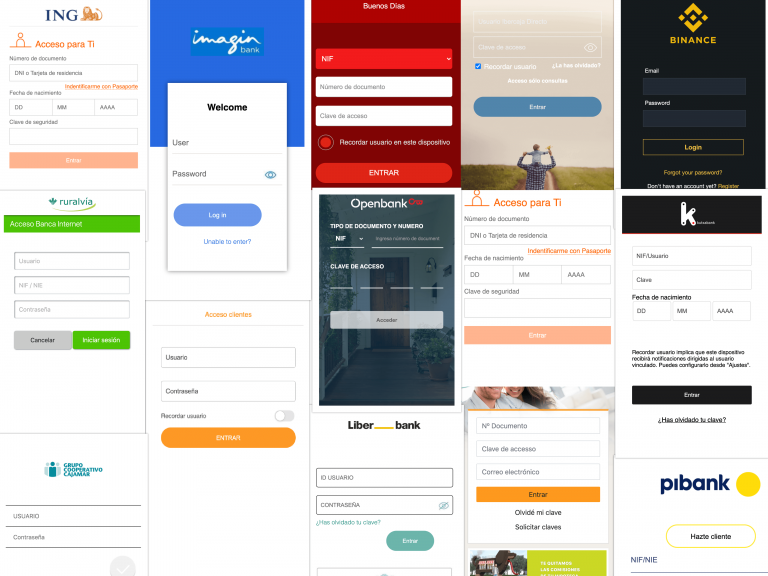
\includegraphics[scale=0.51]{infected.png}

\end{center}


\end{frame}
\section{Technische Analyse}
\begin{frame}{Technische Analyse}
 - Die Apk ist komplett in Java geschrieben\\
 - Läuft ab Android Version 4.1.2\\
 - Verwendet String Obfuscation um Reverse Engineering zu erschweren!\\
 - Über 30 Kommandos kann der C\&C Server mit dem Gerät Kommunizieren!
\end{frame}
\begin{frame}
\begin{shaded}
\#Kommandos von dem C\&C Server an das Gerät

GET\_CONTACTS - Schicke Kontakte an den Server.\\
RETRY\_INJECT - Versuche erneut die Anwendung zu infizieren\\
BLOCK - Jegliche Kommunikation blocken\\
UNINSTALL\_APP - Deinstalltion der Malware\\
SEND\_SMS - Versenden von SMS\\
DISABLE\_PLAY\_PROTECT - Den Virenschutz des Google Play stores deaktivieren\footnote{https://raw.githubusercontent.com/prodaft/malware-ioc/master/FluBot/FluBot.pdf}
\end{shaded}
\end{frame}

\begin{frame}{Netzwerkstrukur}
- Flubot verwendet gekapperte Webeiten als Hosts.\\
- Über 200 betroffene Blogs!\\
- Keine Feste Domain oder IP!\\
- Domaingenerierung anhand des DGA\\
- Auflösung über DNS über HTTPS\\
- Nutzt Services wie dns.google
\end{frame}
\begin{frame}
\begin{center}
 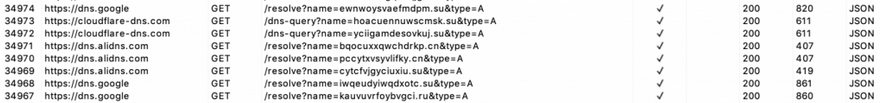
\includegraphics[scale=0.51]{dns.png}

\end{center}
\end{frame}
\section{Conclusion}
\begin{frame}{Conclusion}
 - Pishing nach wie vor größte Bedrohungslage\\
 - Keine technische Lösung!\\
 - Geringer schutz durch 2FA möglich!\\
 - Nachhaltiger Schutz bzw. Bekämpfung nur durch bessere Aufklärung und Bildung möglich!
\end{frame}
\section{Quellen}
\begin{frame}{Quellen}
https://de.statista.com/statistik/daten/studie/1235321\\
https://de.statista.com/themen/1355/android/\\
https://www.telekom.com/en/blog/group/article/flubot-under-the-microscope-636368\\
https://www.telekom.com/en/blog/group/article/flubot-under-the-microscope-636368\\
https://www.computerbild.de/artikel/cb-News-Sicherheit-Flubot-Gefaehrliche-Android-Malware-verbreitet-sich-ueber-Fake-Patches-30863335.html\\
https://computerwelt.at/news/android-malware-flubot-stuermt-top-ten\\
https://www.telekom.com/en/blog/group/article/flubot-under-the-microscope-636368\\

\end{frame}

\end{document}
